\chapter*{
    \begin{center}
        \vspace{-3cm}
        {\Large Annexe A : Limites de la première version de PENTRA}
    \end{center}
}
\addcontentsline{toc}{chapter}{Annexe A: Limites de la première version de PENTRA}
\vspace{-2.5cm}
\begin{justify}
Cette annexe présente les interfaces et la structure de base de données de la première version de l'application \textbf{PENTRA}. Cette version initiale comporte plusieurs limitations, tant en termes d'expérience utilisateur que d'architecture technique.
    \begin{enumerate}
        \item \textbf{Structure initiale de la base de données:}\\
            La base de données repose uniquement sur deux tables: \texttt{utilisateur} et \texttt{rapport}. Cette conception limite les possibilités d’extension et de gestion fine des tests.
            \begin{figure}[H]
                \centering
                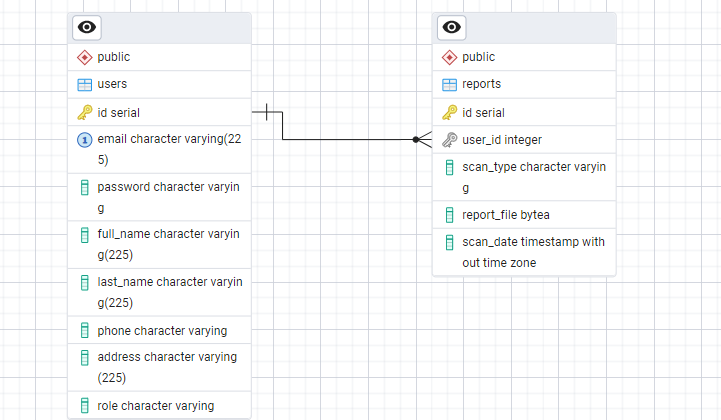
\includegraphics[width=0.8\linewidth]{Annexe/PENTRA-V1/db.PNG}
                \caption{\centering Structure initiale de la base de données de l'application PENTRA}
                \label{fig:PENTRA-db-initial}
            \end{figure}
            \vspace{-0.5cm}
    \item \textbf{Interfaces de la version initiale:}\\
    Les interfaces de cette version présentent certaines limites tant sur le plan ergonomique que fonctionnel. Les figures suivantes illustrent les principales fonctionnalités de l’application. 
        \begin{figure}[H]
            \centering
            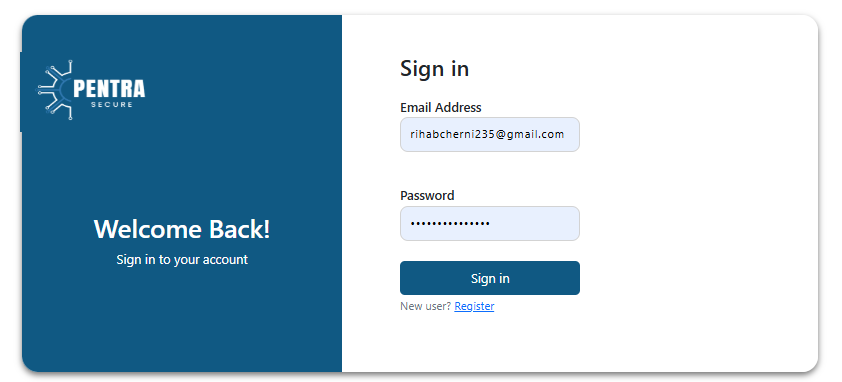
\includegraphics[width=0.8\linewidth]{Annexe/PENTRA-V1/3.PNG}
            \caption{\centering Interface de connexion (PENTRA)}
            \label{fig:PENTRA-V1-3}
        \end{figure}
          \vspace{-0.3cm}
        \begin{figure}[H]
            \centering
            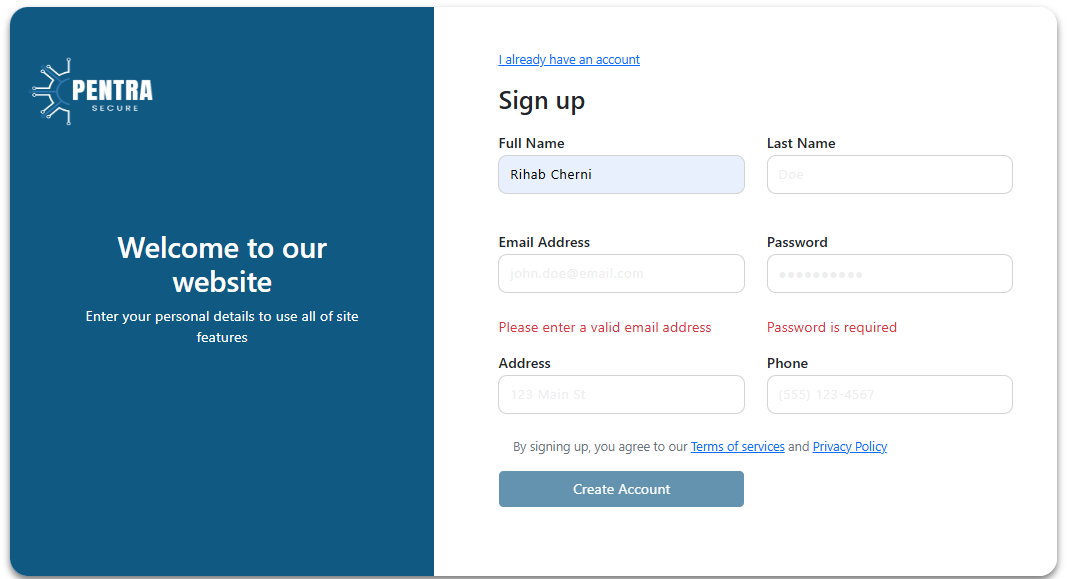
\includegraphics[width=0.8\linewidth]{Annexe/PENTRA-V1/2.PNG}
            \caption{\centering Interface d'inscription (PENTRA)}
            \label{fig:PENTRA-V1-2}
        \end{figure}
        \vspace{-0.3cm}
        \begin{figure}[H]
            \centering
            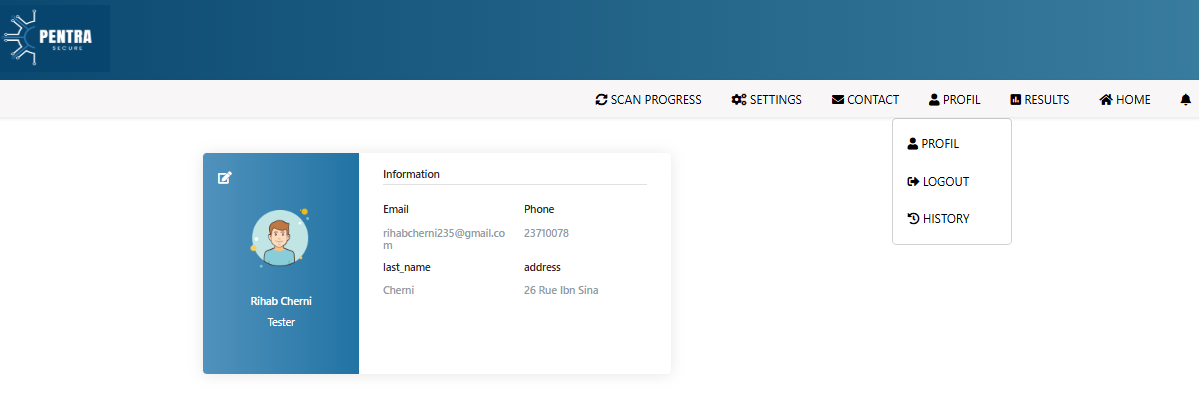
\includegraphics[width=0.8\linewidth]{Annexe/PENTRA-V1/13.PNG}
            \caption{\centering Interface de profil utilisateur}
            \label{fig:PENTRA-V1-11}
        \end{figure}
        \vspace{-0.3cm}
        \begin{figure}[H]
            \centering
            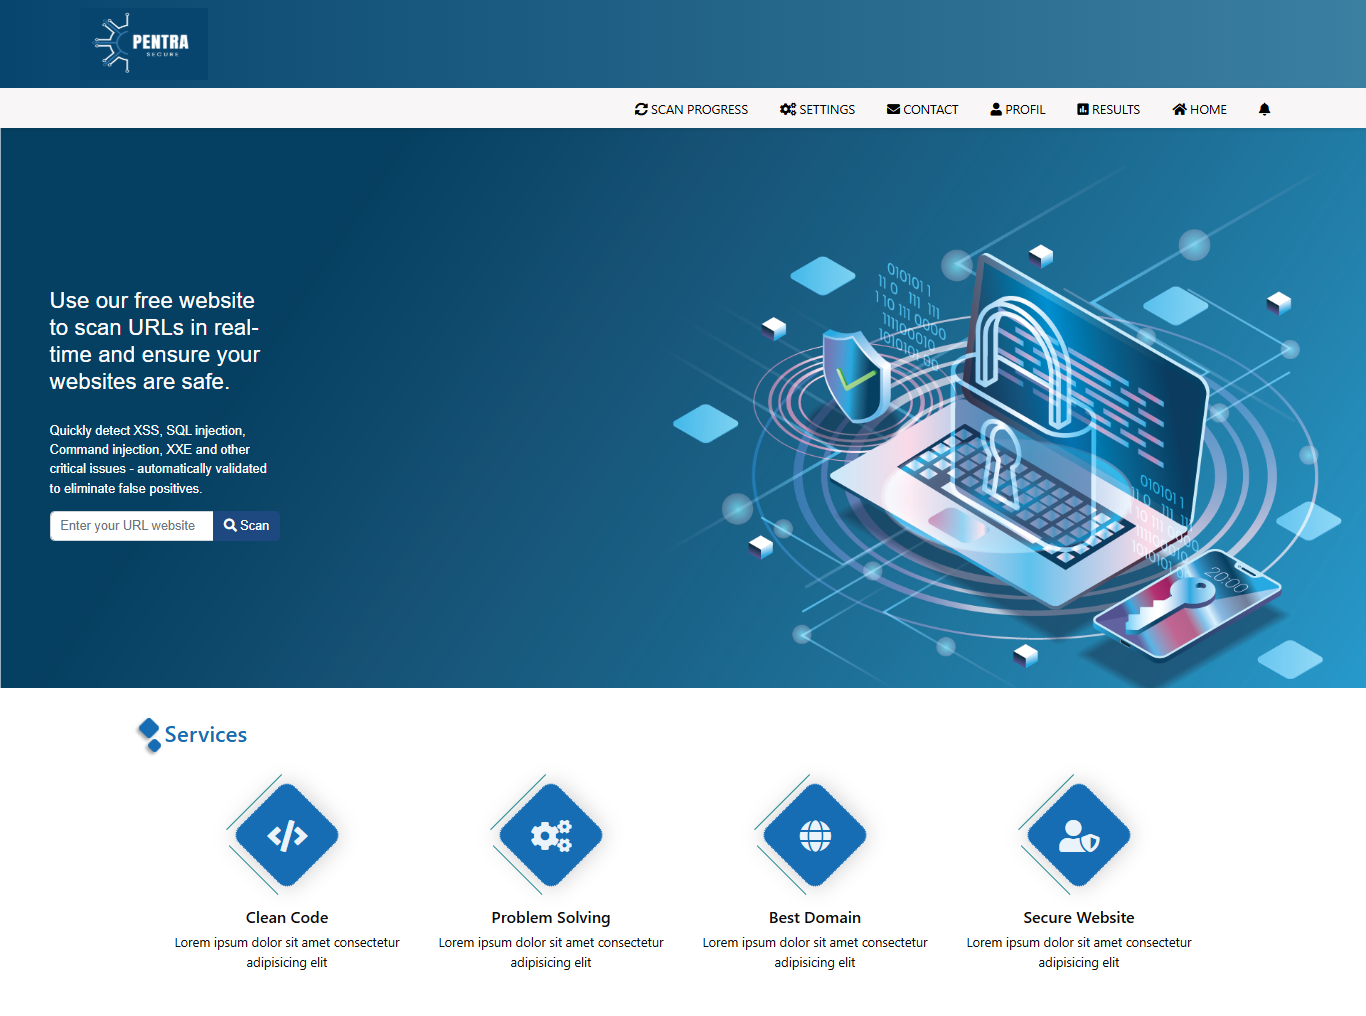
\includegraphics[width=0.8\linewidth]{Annexe/PENTRA-V1/4.png}
            \caption{\centering Interface de lancement du scan de test de pénétration (PENTRA)}
            \label{fig:PENTRA-V1-4}
        \end{figure}
        \vspace{-0.3cm}
        \begin{figure}[H]
            \centering
            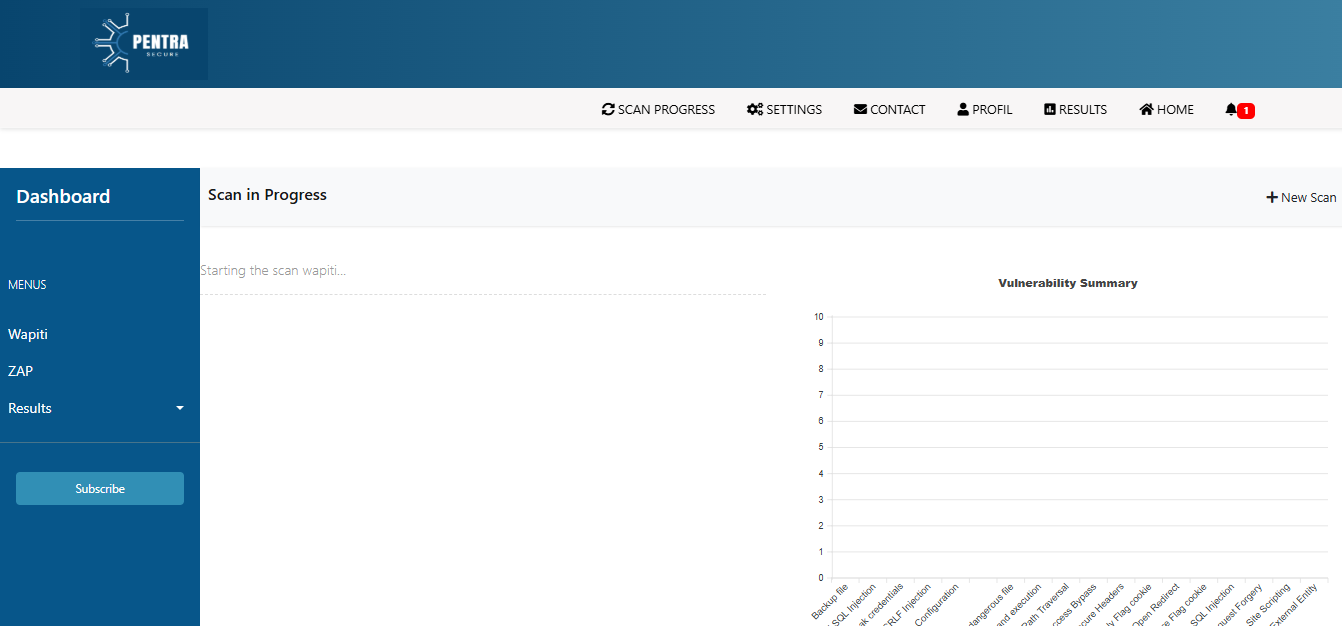
\includegraphics[width=0.8\linewidth]{Annexe/PENTRA-V1/5.PNG}
            \caption{\centering Interface de progression du scan avec Wapiti (PENTRA)}
            \label{fig:PENTRA-V1-5}
        \end{figure}
        \vspace{-0.3cm}
        \begin{figure}[H]
            \centering
            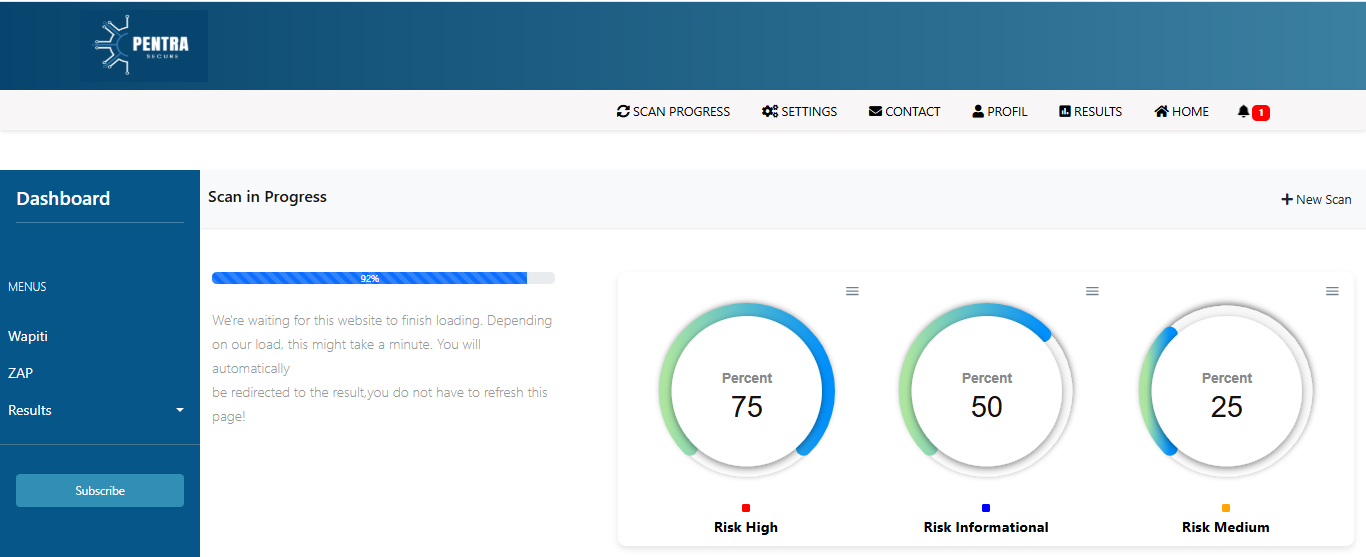
\includegraphics[width=0.8\linewidth]{Annexe/PENTRA-V1/6.PNG}
            \caption{\centering Interface de progression du scan avec OWASP ZAP (PENTRA)}
            \label{fig:PENTRA-V1-6}
        \end{figure}
        \vspace{-0.3cm}
        \begin{figure}[H]
            \centering
            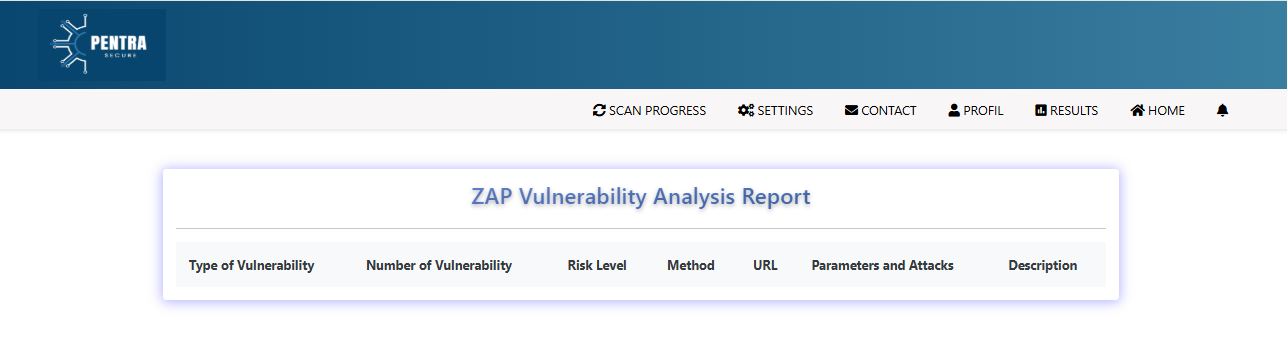
\includegraphics[width=0.8\linewidth]{Annexe/PENTRA-V1/7.PNG}
            \caption{\centering Interface du tableau de résultats du scan avec OWASP ZAP (PENTRA)}
            \label{fig:PENTRA-V1-7}
        \end{figure}
        \vspace{-0.3cm}
        \begin{figure}[H]
            \centering
            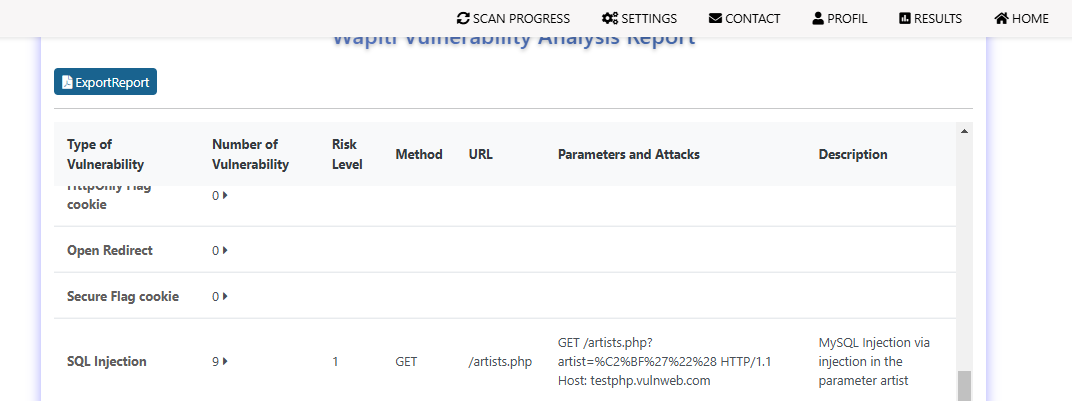
\includegraphics[width=0.8\linewidth]{Annexe/PENTRA-V1/8.PNG}
            \caption{\centering Interface du tableau de résultats du scan avec Wapiti (PENTRA)}
            \label{fig:PENTRA-V1-8}
        \end{figure}
        \vspace{-0.8cm}
        \begin{figure}[H]
            \centering
            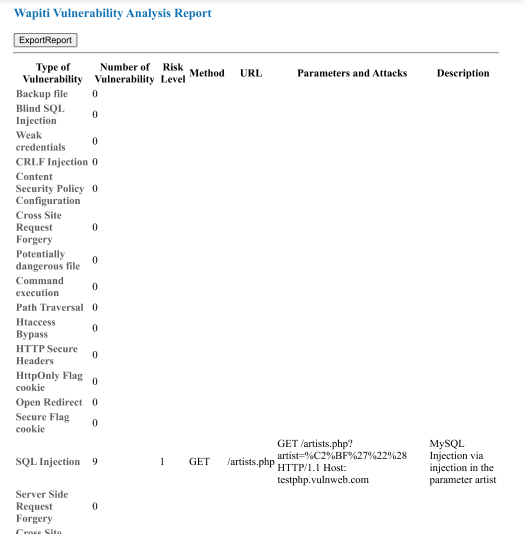
\includegraphics[width=0.8\linewidth]{Annexe/PENTRA-V1/9.PNG}
            \caption{\centering Rapport PDF des vulnérabilités détectées par Wapiti (PENTRA)}
            \label{fig:PENTRA-V1-9}
        \end{figure}
        \vspace{-0.5cm}
        \begin{figure}[H]
            \centering
            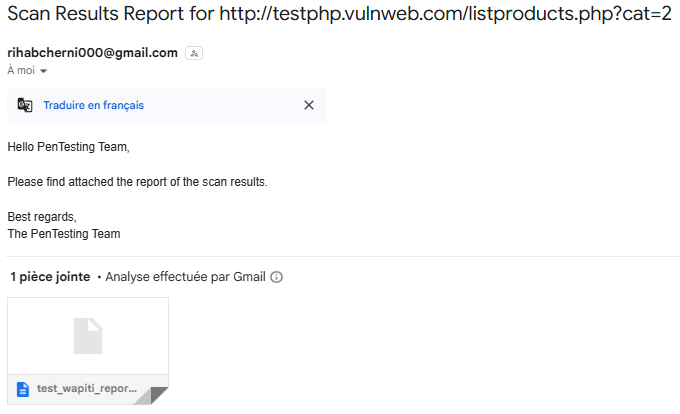
\includegraphics[width=0.8\linewidth]{Annexe/PENTRA-V1/email.PNG}
            \caption{\centering Rapport des vulnérabilités détectées envoyé par e-mail (PENTRA)}
            \label{fig:PENTRA-V1-email}
        \end{figure}
        \vspace{-0.3cm}
        \begin{figure}[H]
            \centering
            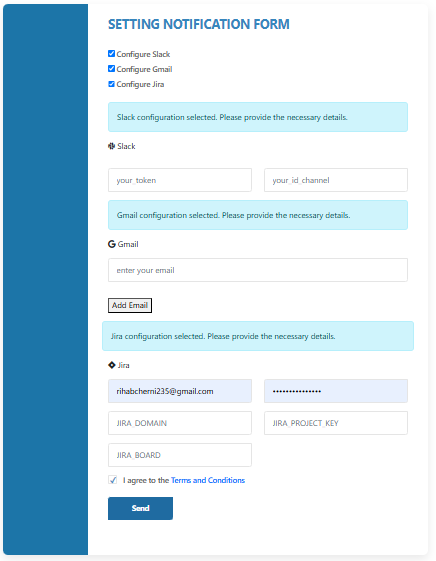
\includegraphics[width=0.8\linewidth]{Annexe/PENTRA-V1/11.PNG}
            \caption{\centering Interface de configuration des paramètres d'envoi des rapports (PENTRA)}
            \label{fig:PENTRA-V1-10}
        \end{figure}
        \vspace{-0.8cm}
        \begin{figure}[H]
            \centering
            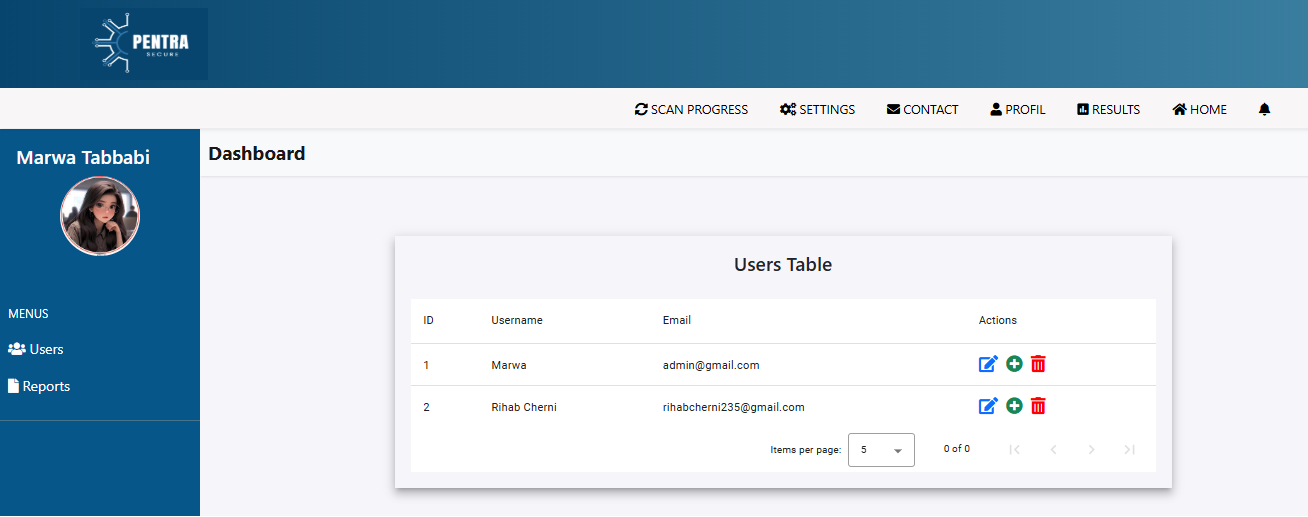
\includegraphics[width=0.8\linewidth]{Annexe/PENTRA-V1/14.png}
            \caption{\centering Interface de gestion des utilisateurs par l'administrateur (PENTRA)}
            \label{fig:PENTRA-V1-12}
        \end{figure}
         \vspace{-0.8cm}
        \begin{figure}[H]
            \centering
            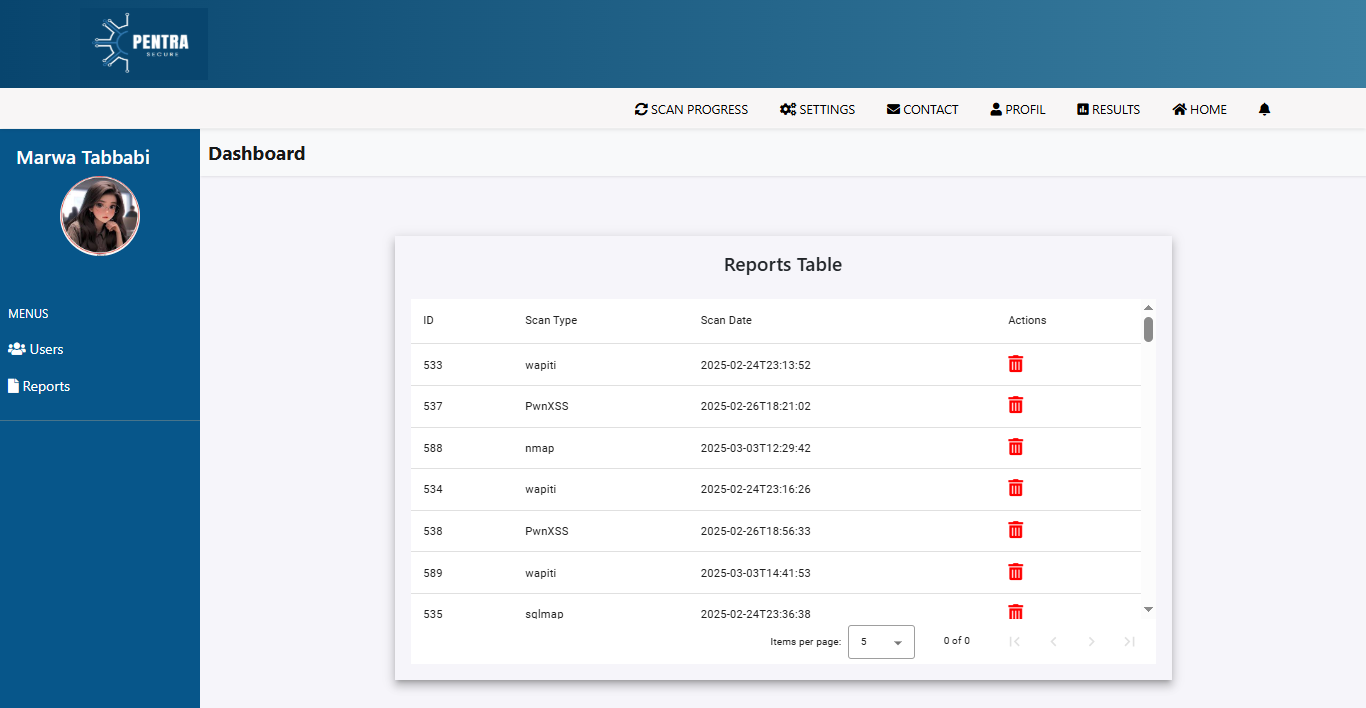
\includegraphics[width=0.8\linewidth]{Annexe/PENTRA-V1/15.png}
            \caption{\centering Interface de gestion des rapports de scan par l'administrateur (PENTRA)}
            \label{fig:PENTRA-V1-13}
        \end{figure}
        \vspace{-0.3cm}
        \end{enumerate}
        En résumé, la première version de l'application \textbf{PENTRA} présente plusieurs limites, tant au niveau de la structure de données que de l’ergonomie des interfaces. Une refonte globale s’impose afin d’améliorer la navigation, l’esthétique et l’intuitivité de l’application. Cette nouvelle version devra également permettre une exploitation plus efficace et complète des données collectées, tout en répondant aux exigences de maintenabilité et d’évolutivité du projet.
 \end{justify}
